\documentclass[border=10pt]{standalone}

\usepackage{tikz}
\usepackage{tikzsymbols}
\usetikzlibrary{calc,patterns,shapes.geometric}

\def\centerarc[#1](#2)(#3:#4:#5){\draw[#1] ($(#2)+({#5*cos(#3)},{#5*sin(#3)})$) arc (#3:#4:#5);}

\begin{document}
	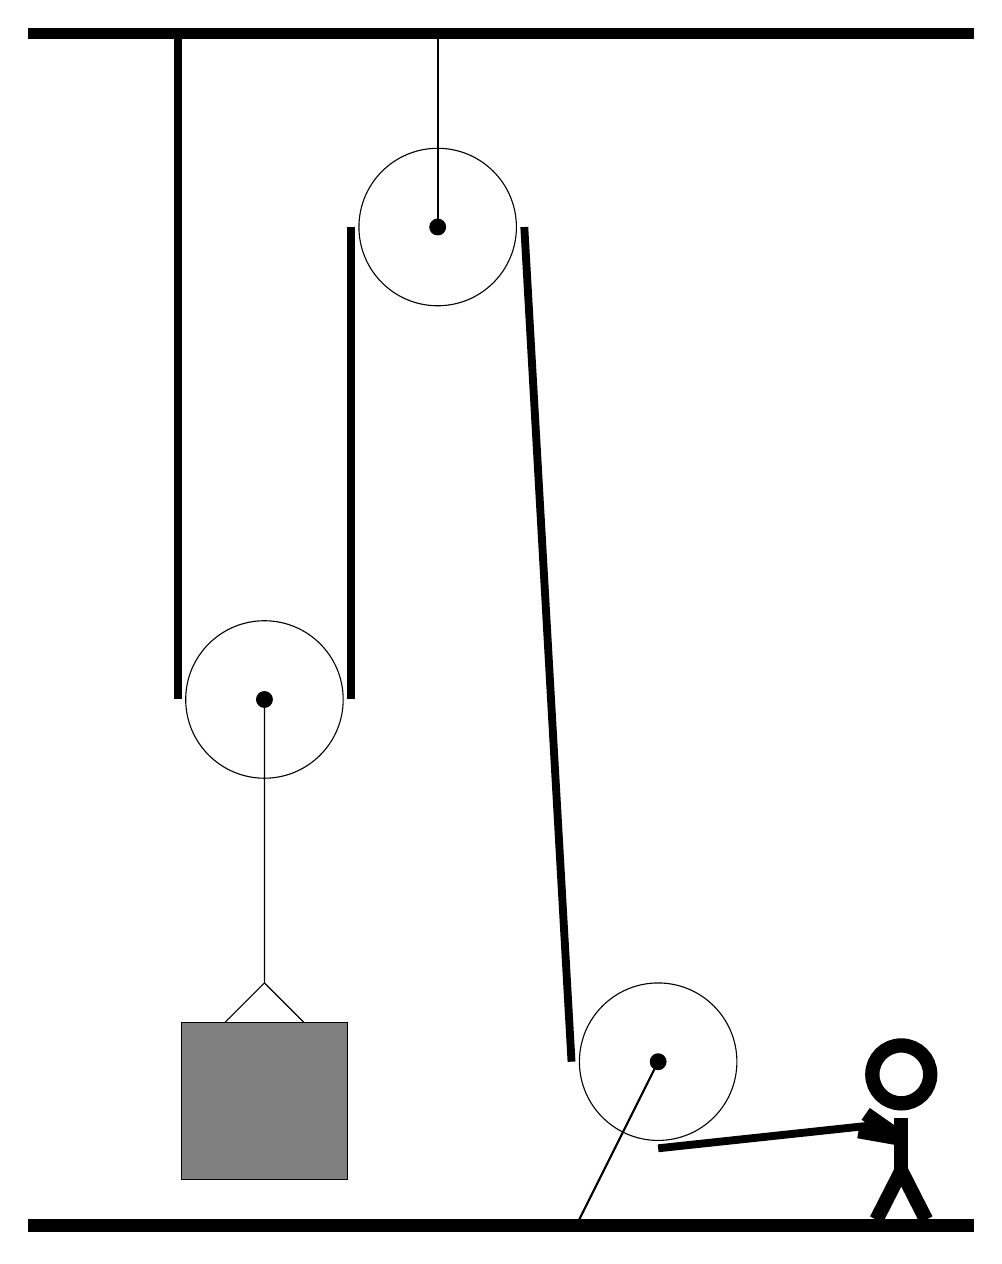
\begin{tikzpicture}
		%%%%% START %%%%%
		\draw[fill=black] (-2, 12) rectangle (10, 12.125);
		
		\draw (3.2, 9.6) circle (1);
		\draw[fill=black] (3.2, 9.6) circle (0.1);
		\draw[thick] (3.2, 9.6) -- (3.2, 12);
		
		\draw (6, -1) circle (1);
		\draw[fill=black] (6, -1) circle (0.1);
		\draw[thick] (6, -1) -- (5, -3);
		
		\draw (1, 3.6) circle (1);
		\draw[fill=black] (1, 3.6) circle (0.1);
		
		\draw (1, 3.6) -- (1, 0) -- (0.5, -0.5);
		\draw (1, 0) -- (1.5, -0.5);
		\draw[fill=black!50] (-0.05, -0.5) rectangle (2.05, -2.5);
		
		\draw[line width=1mm] (-0.1, 12) -- (-0.1, 3.6);
		\centerarc[line width=1mm](1, 3.6)(180:360:1.1);
		\draw[line width=1mm](2.1, 3.6) -- (2.1, 9.6);
		\centerarc[line width=1mm](3.2, 9.6)(0:180:1.1);
		\draw[line width=1mm](4.3, 9.6) -- (4.9, -1);
		\centerarc[line width=1mm](6, -1)(180:270:1.1);
		\draw[line width=1mm](6, -2.1) -- (8.8, -1.8);
		
		\node at (9, -1.9) {\Strichmaxerl[10][-35][170]};
		
		\draw[fill=black] (-2, -3) rectangle (10, -3.15);
		%%%%% END %%%%%
	\end{tikzpicture}
\end{document}